\documentclass[10pt,twocolumn,letterpaper]{article}
\usepackage[final]{cvpr}

% Standard packages
\usepackage{graphicx}
\usepackage{amsmath,amssymb}
\usepackage{booktabs}
\usepackage{xcolor}
\usepackage{hyperref}
\usepackage{tikz}
\usetikzlibrary{positioning,arrows.meta,shapes.geometric,calc}

% Bibliography
\usepackage[numbers,sort&compress]{natbib}
\bibliographystyle{ieeenat_fullname}

\begin{document}

% ============================================================
\title{PIDNet-S with Copy-Paste Obstacle Augmentation}
\author{JM Raitz -- RH Cheppally}
\maketitle
\thispagestyle{empty}

% ============================================================
% Single-column technical report (~half page / one column)
% Submission: #17029 on leaderboard (Q = 52.1)
% ============================================================

\noindent\textbf{Method name:} PIDNet-S with Copy-Paste Obstacle Augmentation.

\noindent\textbf{Submission:} \#17029 on the challenge leaderboard (Q\,=\,52.1, mIoU\,=\,94.4\%, F1\,=\,55.2\%).

\vspace{0.3em}
\noindent\textbf{Architecture.}
We use PIDNet-S~\cite{xu2023pidnet} (\href{https://github.com/XuJiacong/PIDNet}{github.com/XuJiacong/PIDNet}), a lightweight three-branch (Proportional--Integral--Derivative) network with 32 base channels, PPM pooling (96~channels), and a PIDHead decoder (128~channels, 3~classes). The backbone is initialized from ImageNet-1K pretrained weights. We made no architectural modifications---PIDNet-S was selected specifically because its BatchNorm + Conv + ReLU composition quantizes cleanly under the server's INT8 quantization pipeline on the Luxonis RVC4. During our evaluation phase, we found that architectures relying on attention mechanisms (SegFormer) or large-kernel depthwise convolutions (SegNeXt) suffered catastrophic INT8 degradation ($-$67\% to $-$82\% mIoU), making simple convolution-based designs the only viable choice.

\vspace{0.3em}
\noindent\textbf{Training.}
We train at the target resolution of $768 \times 384$ using SGD (lr\,=\,0.133, momentum\,=\,0.9, weight decay\,=\,$5{\times}10^{-4}$) for 15{,}000 iterations with polynomial LR decay (power\,=\,0.9) and a 2{,}500-iteration linear warmup.
Batch size is 320 (160 per GPU). Losses: CrossEntropy ($w$\,=\,0.4), two OHEM losses ($w$\,=\,1.0, threshold\,=\,0.9), and BoundaryLoss ($w$\,=\,20). Augmentations include Large Scale Jittering (ratio $\in [0.5, 2.0]$), random crop, horizontal flip, enhanced photometric distortion (brightness, contrast, saturation, hue, gamma jitter), and reflect padding matching the server preprocessing. Framework: mmsegmentation~\cite{mmseg2020}, PyTorch~2.1.2, CUDA~12.1.

\vspace{0.3em}
\noindent\textbf{Copy-Paste augmentation.}
The key component of our method is a Copy-Paste obstacle augmentation~\cite{ghiasi2021copypaste} using crops extracted from three external maritime datasets: \textbf{WaterScenes}~\cite{yao2024waterscenes}, \textbf{ROSEBUD}~\cite{lambert2022rosebud}, and the night subset of \textbf{MULTIAQUA}~\cite{iancu2024multiaqua}. All three were remapped to the LaRS 3-class schema and deduplicated with perceptual hashing. We mined ${\sim}$30{,}000 obstacle crops (water-adjacent, area 50--100k\,px at target resolution) and stored them in a shared database. During training, with probability 0.7, 1--3 crops are sampled with size-based tier weights (oversampling small obstacles), brightness-matched to the local water region, and pasted before photometric distortion. This approach was motivated by a failure analysis of our Phase~2 baseline server submission and a spatial out-of-distribution study on the LaRS test set, both of which showed that the majority of false negatives involved small or rare obstacle types under unusual lighting---gaps that external maritime datasets could address. An initial run with a shorter schedule (8k iterations) failed due to ``augmentation shock,'' which we resolved by extending to 15k iterations with longer warmup.

\vspace{0.3em}
\noindent\textbf{Datasets.}
LaRS~\cite{zust2023lars} (train: 2{,}605 images) for training; ImageNet-1K for backbone pretraining; WaterScenes, ROSEBUD, and MULTIAQUA\_night as external augmentation sources (crops only, no joint training). No custom-annotated data was used.

\vspace{0.3em}
\noindent\textbf{Hardware \& inference speed.}
Training was performed on 2$\times$ NVIDIA RTX A6000 (48\,GB) with DDP. On the challenge server (Luxonis RVC4, INT8 quantization), our model achieves 67.7\,FPS.

% Optional figure — can be removed to save space
\begin{figure}[t]
\centering
\resizebox{0.95\columnwidth}{!}{%
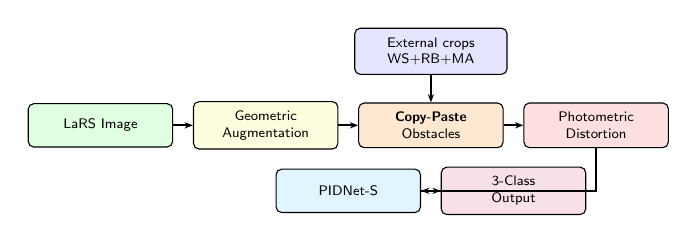
\begin{tikzpicture}[
  box/.style={draw, rounded corners=2pt, minimum height=0.55cm,
              text width=1.6cm, align=center, font=\tiny\sffamily},
  arr/.style={-{Stealth[length=3pt]}, semithick},
  dbbox/.style={draw, rounded corners=2pt, minimum height=0.45cm,
                fill=blue!10, text width=1.7cm, align=center, font=\tiny\sffamily},
]
  \node[box, fill=green!12] (input) {LaRS Image};
  \node[box, fill=yellow!12, right=0.25cm of input] (geom) {Geometric\\Augmentation};
  \node[box, fill=orange!18, right=0.25cm of geom] (cp) {\textbf{Copy-Paste}\\Obstacles};
  \node[box, fill=red!12, right=0.25cm of cp] (photo) {Photometric\\Distortion};
  \node[box, fill=cyan!12, below=0.55cm of $(geom)!0.5!(cp)$] (model) {PIDNet-S};
  \node[box, fill=purple!12, right=0.25cm of model] (out) {3-Class\\Output};
  \node[dbbox, above=0.35cm of cp] (db) {External crops\\WS+RB+MA};
  \draw[arr] (input) -- (geom);
  \draw[arr] (geom) -- (cp);
  \draw[arr] (cp) -- (photo);
  \draw[arr] (db) -- (cp);
  \draw[arr] (photo) |- (model);
  \draw[arr] (model) -- (out);
\end{tikzpicture}%
}
\caption{Training pipeline. WS\,=\,WaterScenes, RB\,=\,ROSEBUD, MA\,=\,MULTIAQUA\_night.}
\label{fig:pipeline}
\end{figure}

% ============================================================
{\small
\bibliography{references}
}

\end{document}
